\documentclass[10pt,a4paper,openany]{report}
\title{Rapport LO21}
\usepackage[spanish]{babel} %Indica que escribiermos en español
\usepackage[utf8]{inputenc} %Indica qué codificación se está usando ISO-8859-1(latin1)  o utf8  
\usepackage{amsmath} % Comandos extras para matemáticas (cajas para ecuaciones,
% etc)
\usepackage{amssymb} % Simbolos matematicos (por lo tanto)
\usepackage{graphicx} % Incluir imágenes en LaTeX
\usepackage{color} % Para colorear texto
\usepackage{subfigure} % subfiguras
\usepackage{float} %Podemos usar el especificador [H] en las figuras para que se
% queden donde queramos
\usepackage{capt-of} % Permite usar etiquetas fuera de elementos flotantes
% (etiquetas de figuras)
\usepackage{sidecap} % Para poner el texto de las imágenes al lado
\sidecaptionvpos{figure}{c} % Para que el texto se alinie al centro vertical
\usepackage{caption} % Para poder quitar numeracion de figuras
\usepackage{commath} % funcionalidades extras para diferenciales, integrales,
% etc (\od, \dif, etc)
\usepackage{cancel} % para cancelar expresiones (\cancelto{0}{x})

\usepackage{anysize} 					% Para personalizar el ancho de  los márgenes
\marginsize{2cm}{2cm}{2cm}{2cm} % Izquierda, derecha, arriba, abajo

\usepackage{appendix}
\renewcommand{\appendixname}{Apéndices}
\renewcommand{\appendixtocname}{Apéndices}
\renewcommand{\appendixpagename}{Apéndices} 

% Para que las referencias sean hipervínculos a las figuras o ecuaciones y
% aparezcan en color
\usepackage[colorlinks=true,plainpages=true,citecolor=blue,linkcolor=blue]{hyperref}
%\usepackage{hyperref} 
% Para agregar encabezado y pie de página
\usepackage{fancyhdr} 
\pagestyle{fancy}
\fancyhf{}
\fancyhead[L]{\footnotesize UTC} %encabezado izquierda
\fancyhead[R]{\footnotesize LO21}   % dereecha
\fancyfoot[R]{\footnotesize Rapport}  % Pie derecha
\fancyfoot[C]{\thepage}  % centro
\fancyfoot[L]{\footnotesize Génie informatique}  %izquierda
\renewcommand{\footrulewidth}{0.4pt}


\usepackage{listings} % Para usar código fuente
\definecolor{dkgreen}{rgb}{0,0.6,0} % Definimos colores para usar en el código
\definecolor{gray}{rgb}{0.5,0.5,0.5} 
% configuración para el lenguaje que queramos utilizar
\lstset{language=Matlab,
	keywords={break,case,catch,continue,else,elseif,end,for,function,
		global,if,otherwise,persistent,return,switch,try,while},
	basicstyle=\ttfamily,
	keywordstyle=\color{blue},
	commentstyle=\color{red},
	stringstyle=\color{dkgreen},
	numbers=left,
	numberstyle=\tiny\color{gray},
	stepnumber=1,
	numbersep=10pt,
	backgroundcolor=\color{white},
	tabsize=4,
	showspaces=false,
	showstringspaces=false}

\newcommand{\sen}{\operatorname{\sen}}	% Definimos el comando \sen para el seno
%en español

\title{Rapport}
\begin{document}

	\begin{center}																		
		\newcommand{\HRule}{\rule{\linewidth}{0.5mm}}									
		\begin{minipage}{\textwidth} \begin{flushleft}
				
\includegraphics[scale = 0.5]{utc_logo.jpg}
		\end{flushleft}\end{minipage}
		\\[1.0cm]
		\textsc{\huge Université de Techonologie\\ \vspace{5px} de Compiègne}\\[1.0cm]	
		\textsc{\LARGE\textbf{LO21}}\\[1.0cm]													
		\begin{minipage}{0.9\textwidth} 
			\begin{center}																	
				\textsc{\LARGE Rapport}
			\end{center}
		\end{minipage}\\[0.5cm]
		\vspace*{1cm}
		\HRule \\[0.4cm]
		{ \huge \bfseries Projet Trésorerie}\\[0.4cm]
		\HRule \\[1.5cm]
		\begin{minipage}{0.3\textwidth}
			\begin{flushleft} \large
				% Aqui a continuación pongan los nombres de los integrantes
				\emph{Autores:}\\
				BENDYNA Lucas\\
				GOURET Mathilde\\
				RAMIREZ Brenda\\
				XIE Sihan\\	 
			\end{flushleft}
		\end{minipage}					
	\end{center}							 
	\newpage								
	\tableofcontents 
	\newpage
	\section{Résumé de l'application.}
	
	\subsection{Opérations implémentes}
	
	\subsubsection{Connexion}
	Connexion permet d'accéder aux informations de la base de données déconnecter l'utilisateur.
	
	\subsubsection{Comptes}
	Les comptes peuvent être classifiées en catégories:
	\begin{itemize}
		\item Actifs 
		\item Passifs
		\item Recettes
		\item Dépenses
	\end{itemize}
	
	Chacune a la possibilité d'ajouter une compte, l'éditer, réaliser une transaction et d'afficher ces transactions.
	\textbf{Ajouter un compte} prends en compte:
	\begin{itemize}
		\item Nom 
		\item Compte père
		\item S'il est virtuel ou pas
		\item Solde initial
		\item Compte de capitaux propre à utiliser
	\end{itemize}
	\textbf{Ajouter une transaction} contient:
	\begin{itemize}
		\item Réference
		\item Intitulé
		\item Comptes
		\item Crédit
		\item Débit
	\end{itemize}
	\subsection{Opérations non implémentes}
	\begin{itemize}
		\item LOGIN : Il n'est pas possible d'ajouter un compte dans l'application.
		\item COMPTES: L'application manipule une seule compte

	\end{itemize}
	\subsubsection{Transactions}
	L'onglet Transactions affiche les transactions effectués. Il est implémenté avec deux boutons, une pour ajouter une transaction avec le même format de celui-ci des comptes et l'enregistrement pour actualiser l'affichage.
	
	\subsubsection{Rapports}
	Rapports représente le Bilan (d'actifs et passifs), et le Compte de résultat (). Bilan affiche les comptes et ses montants. D'autre côté le compte de résultat affiche le total recettes,le total dépenses et le perte d'aujourd'hui
	Cet onglet ne peut pas montrer l'option \textbf{clôture}
	
	\subsubsection{Clôture}
	La clôture remettre à zéro les comptes de recettes et dépenses par l'intermediaire d'un compte résultat et transfère la différence ver s le compte excédent ou déficit au contraire
	\subsubsection{Déconnexion}
	Déconnexion permet de déconnecter l'utilisateur
	
	
	\subsection{Description de l'architecture}
	
	\begin{itemize}
		\item Base de données:Nous avons choisi une base de données plutôt qu'un table ou document à raison qu'ils sont bien plus efficaces lorsqu'il s'agit de retrouver des informations. Il est possible de les afficher sous forme de formulaires dans l'interface graphique, permettant d'accéder en toute liberté à tous les détails enregistrés.
		\item Qt Designer UI: Implémentation de UI pour représenter l'interface graphique de l'application à travers d'un éditeur visuel qui permet de positionner et ajuster les widgets plus facilement et comme nous le souhaitons.

	\end{itemize}
	
	
	\subsection{Argumentation de l'architecture permettant plus facilement les évolutions}
	
	\subsection{Base de données}	
	 De plus, le choix de PostgreSQL a été parce qu'il est le plus complet aujourd'hui, permet de sauvegarder et restaurer des backups facilement, capable de manipuler gros volumes de données.
	
	\subsection{Qt Designer UI}
	Les fichiers d'interface utilisateur de Qt Designer représentent l'arborescence des widgets du formulaire au format XML. Les formulaires peuvent être traités:
	
	Au moment de la compilation, ce qui signifie que les formulaires sont convertis en code C ++ qui peut être compilé.
	Au moment de l'exécution, ce qui signifie que les formulaires sont traités par la classe QUiLoader qui construit dynamiquement l'arborescence des widgets lors de l'analyse du fichier XML.

	\section{Planning du projet}
	
	Le planning du projet a été planifié à travers d'un diagramme de GANTT réaliser pour tous les membres du groupe
	
	\begin{figure}[H]
		\begin{center}
			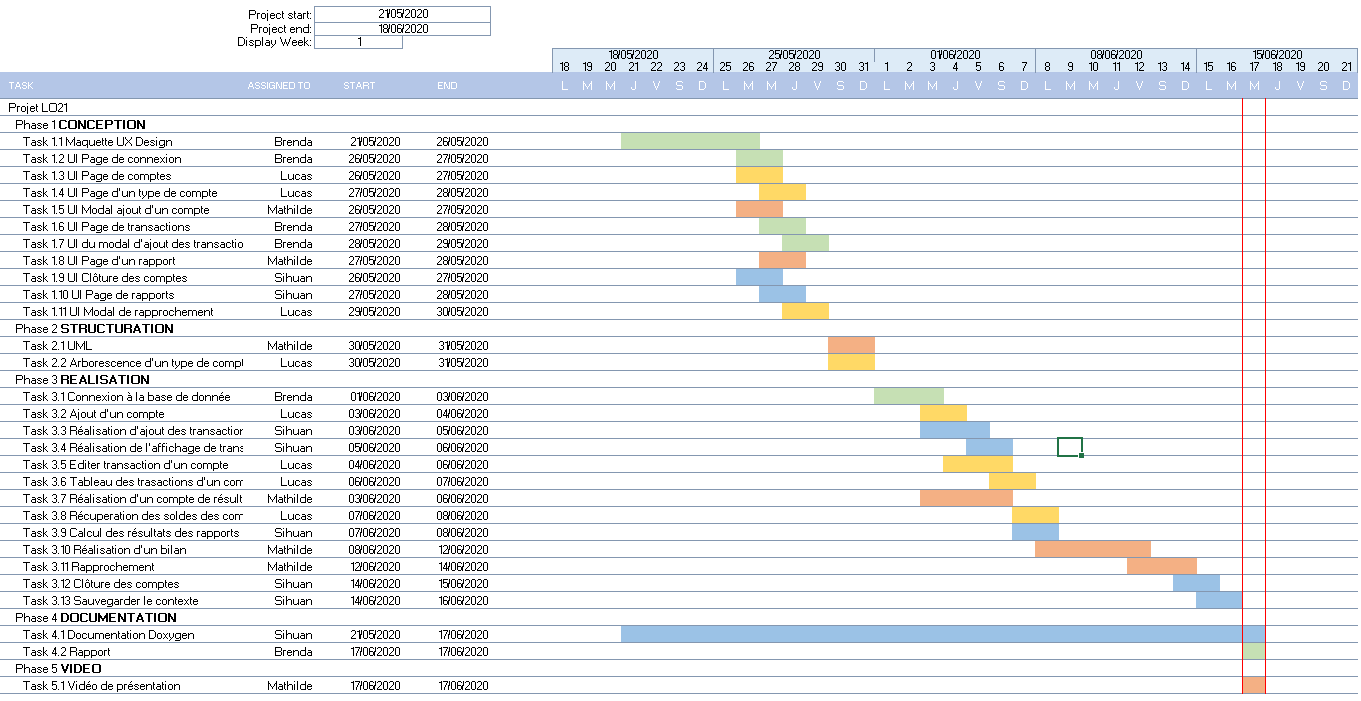
\includegraphics[width = 1\textwidth]{GANTT.PNG}
			\captionof{figure}{\label{fig:silla3ruedas}Silla de ruedas para subir escaleras} 
		\end{center} 
	\end{figure}
	
	
	\section{Contribution personnelle des membres du groupe}

	\subsection{BENDYNA Lucas}
	\begin{itemize}
		\item UI Modal de rapprochement
		\item Rapprochement d'un compte
		\item UI Page de comptes
		\item Récuperation des soldes des comptes
		\item UI Page d'un type de compte
		\item Arborescence d'un type de compte
		\item Tableau des transactions d'un compte
		\item Ajout d'un compte
		\item Éditer Transaction d'un compte
		\item Vidéo de présentation	
	\end{itemize}
	\subsection{GOURET Mathilde}
	\begin{itemize}
		\item Réalisation d'un bilan
		\item Réalisation d'un compte de résultat
		\item UI Page d'un rapport
		\item UI Modal Ajout d'un compte
		\item UML 
		\item Rapprochement	
	\end{itemize}
	\subsection{RAMIREZ Brenda}
	\begin{itemize}
		\item UI Page de connexion
		\item Connexion à la base de donnée
		\item Maquette UX Design
		\item UI du modal d'ajout des transactions
		\item UI Page de transactions
		\item Rapport
	\end{itemize}
	\subsection{XIE Sihuan}
	\begin{itemize}
		\item Documentation Doxygen
		\item UI Page des rapports
		\item Calcul des résultats des rapports à l'instant présente
		\item UI Clôture des comptes
		\item Clôture des comptes
		\item Réalisation d'ajouts des transactions
		\item Réalisation de l'affichage de transaction
	\end{itemize}

	\section{Annexes}
	\subsection{Installation base de données}
	Instructions avant le démarrage du projet:
	\begin{itemize}
		\item Vous devrez installer  \href{https://www.postgresql.org/download/}{PostgresSQL} en suivant les instructions de ce \href{https://www.veremes.com/installation-postgresql-windows}{lien}
		Nous vous recommandons de choisir le mot de passe: \textbf{luluben08}. Au contraire vous devrez modifier le mot de passe directement dans le fichier \textbf{databasemanager.cpp} sur la partie du code \textbf{this -$>$ db.setPassword} en ajoutant votre mot de passe. Après l'installation vous démarrerez PostgreSQL 
		\begin{figure}[H]
			\begin{center}
				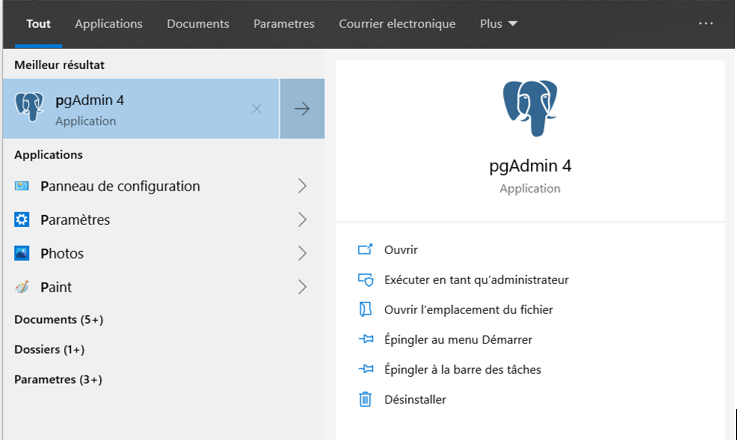
\includegraphics[width = 1\textwidth]{Demarrer_Postgres.PNG}
				\captionof{figure}{\label{fig:silla3ruedas}Silla de ruedas para subir escaleras} 
			\end{center} 
		\end{figure}
	
		Vous introduirez le mot de passe et ensuite vous cliquerez sur Query Tool pour coller le code dans du fichier \textbf{script.sql}, de plus vous devrez ajouter l'instruction \textbf{INSERT INTO public.association (identifiant, mot\_de\_passe) VALUES ('user','password');} à la fin en substituant votre propres données de user et passeword. Finalement l'exécuter . 
		\begin{figure}[H]
			\begin{center}
				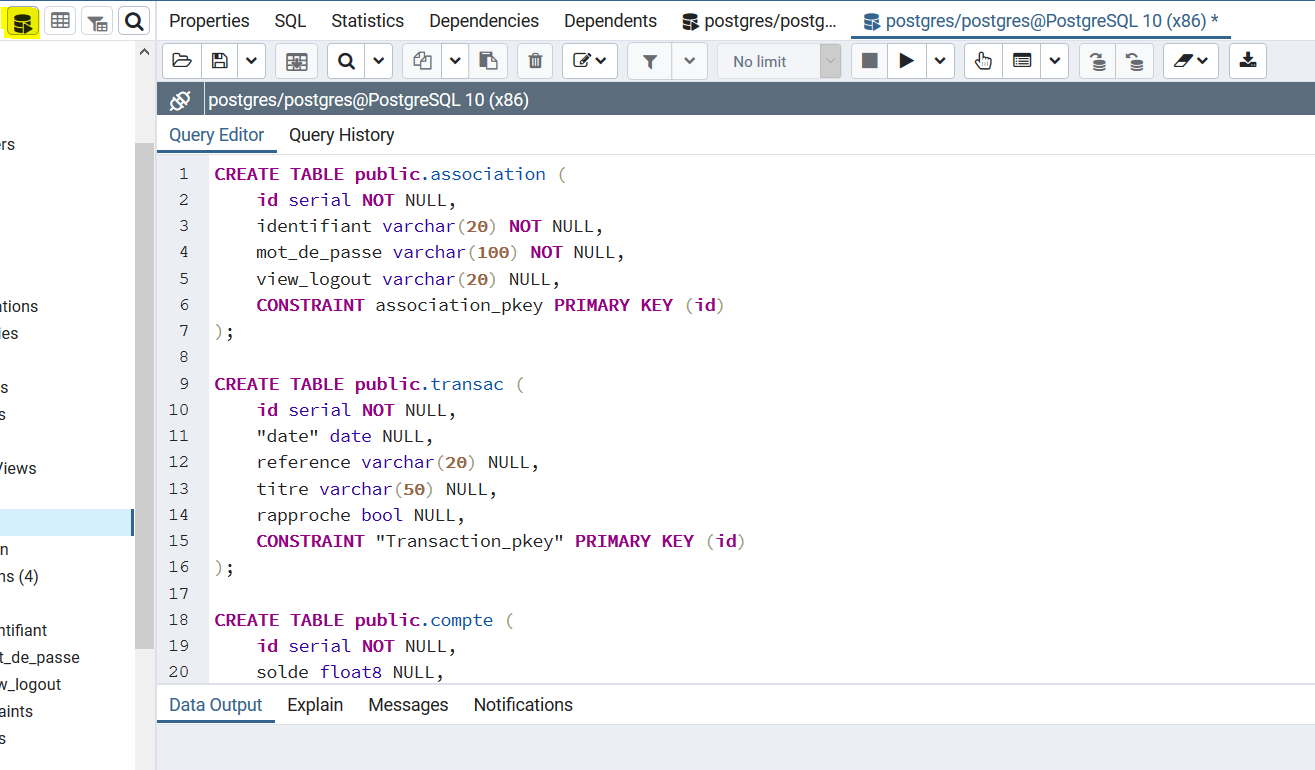
\includegraphics[width = 1\textwidth]{Ajouter_base_de_donnees.PNG}
				\captionof{figure}{\label{fig:silla3ruedas}Silla de ruedas para subir escaleras} 
			\end{center} 
		\end{figure}
		

		\item Vous devrez vérifier la connexion entre Qt et PostgreSQL en cliquant sur l'onglet \textbf{Path} de \textbf{Environnement de Compilation}. Path doit contenir où se localise le fichier bin et lib de PostgresSQL? pour exemple: \textbf{C:$\setminus$ Program Files (x86)$\setminus$ PostgreSQL$\setminus$ 10 $\setminus$ bin}
		\begin{figure}[H]
			\begin{center}
				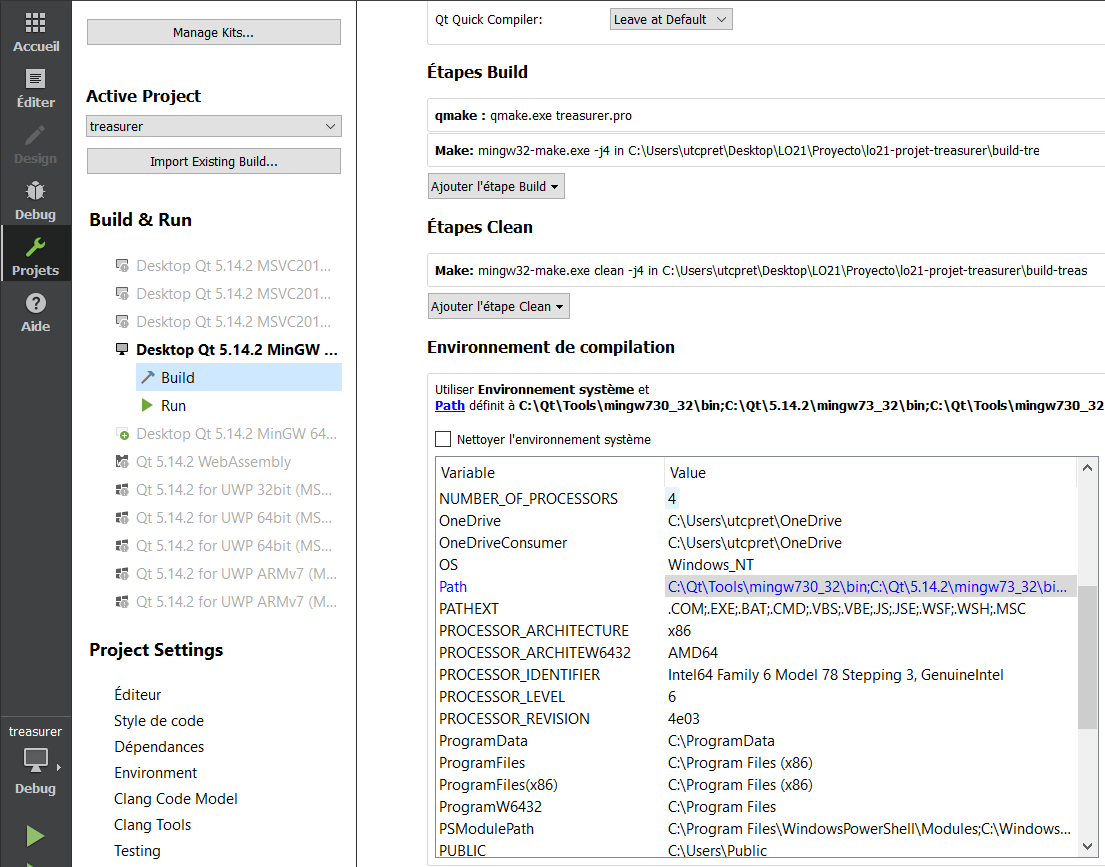
\includegraphics[width = 1\textwidth]{Configuration_Build.PNG}
				\captionof{figure}{\label{fig:silla3ruedas}Silla de ruedas para subir escaleras} 
			\end{center} 
		\end{figure}
	\end{itemize}
	
	
\end{document}